\documentclass[conference]{IEEEtran}
\IEEEoverridecommandlockouts

% Core IEEE and math packages
\usepackage{cite}
\usepackage{amsmath,amssymb,amsfonts}

% Algorithms and figures
\usepackage{algorithm}
\usepackage{algorithmic}
\usepackage{graphicx}
\usepackage{float}

% Text and color
\usepackage{textcomp}
\usepackage{xcolor}

% Tables and layout
\usepackage{booktabs}
\usepackage{tabularx}
\usepackage{url}
\usepackage{subcaption}
\usepackage[compatibility=false]{caption}
\usepackage{comment}
% Symbols and ticks
\usepackage{pifont}

% Diagrams
\usepackage{tikz}
\usetikzlibrary{shapes.geometric, arrows, positioning}

% Custom commands
\newcommand{\cmark}{\ding{51}}% ✓
\newcommand{\xmark}{\ding{55}}% ✗
\def\BibTeX{{\rm B\kern-.05em{\sc i\kern-.025em b}\kern-.08em
    T\kern-.1667em\lower.7ex\hbox{E}\kern-.125emX}}

\begin{document}

\title{In a CIGRE MV Benchmark Redispatch Audit, Operating State Dominates Event Magnitude for Voltage-Limit Violations}

\author{\IEEEauthorblockN{Clifford Omari Ondieki}
\IEEEauthorblockA{\textit{IEEE} \\
Member, Berlin, Germany \\
ondiekiclifford05@gmail.com}
\and
\IEEEauthorblockN{Tianxiang Lu}
\IEEEauthorblockA{\textit{IU International University for Applied Science} \\
Erfurt, Germany \\
tianxiang.lu@iu.org}
}

\maketitle

% --- ABSTRACT ---
\begin{comment}
\begin{abstract}
Verifying that a redispatch instruction keeps a distribution feeder within voltage limits requires a full AC power-flow solve, too slow to run on every event in real time; a cheap, magnitude-based screen is the natural alternative, but how much it actually misses is rarely measured directly. We report an exhaustive empirical audit -- not an estimate -- of one such screen, evaluated against one year of real German TSO redispatch instructions ($N=20{,}586$, seed$=42$) on the CIGRE MV benchmark network. Solving AC power flow for every event, not a sample, we find magnitude-only screening achieves only $15.5\%$ recall (239 of 1,544 confirmed voltage-limit violations) at $5.9\%$ precision -- roughly 94\% of the AC validations it triggers find nothing. A fixed-load control experiment shows why: none of the 4,055 %highest-magnitude events 
events flagged by the magnitude/step-change screen violates without background loading variation, and a regression confirms loading dominates voltage ($r=-0.99$) far more than event magnitude ($r=0.06$). Independent, real SimBench load profiles reproduce this correlation ($r=-0.99$) but find zero violations at native scale -- the evaluation regime that does produce violations is a documented, curated overload $26\%$ above this network's own specified peak, not typical operation. Sweeping a real load shape transparently against this network's own peak locates the onset of violations at $1.35\times$; a genuinely out-of-sample, a deliberately simple diagnostic regression catches only $21$--$26\%$ of violations near this onset but $74\%$ once conditions are pushed to $1.75\times$ -- state-aware screening helps substantially, but mainly under severe stress, not near onset. An earlier in-sample evaluation suggesting near-complete recall was discarded after leakage was identified; all results reported here use the corrected, out-of-sample protocol. Selective AC validation itself is computationally cheap: after deduplicating redundant solves and separating one-time JIT compilation from steady-state cost, %the pipeline misses its 20\,ms software deadline on 1 of 4,055 critical events (0.025\%) across five independent runs
each of five independent runs exceeds the 20\,ms software-latency threshold on 1 of 4,055 critical events (0.025\% per run)-- a latency characterization on one machine, not a real-time guarantee.
\end{abstract}
\end{comment}

\begin{abstract}
Fast screening of voltage-limit violations is attractive for event-driven grid monitoring, but redispatch event information alone is an inadequate proxy for electrical stress. We evaluate this using 20,586 German redispatch records as an event stream mapped onto the CIGRE MV benchmark network. An event-only screen flags 4,055 events but recovers only 15.5\% of confirmed violations, with 5.9\% precision. A fixed-load control produces no violations under the same flagged events, while background loading shows a strong correlation with minimum voltage ($r=-0.99$), compared with $r=0.06$ for redispatch magnitude. This identifies operating state as the dominant explanatory factor in the benchmark and motivates state-aware screening. A held-out, population-separated diagnostic regression recovers 20.5--26.0\% of violations near the onset region and 74.3\% under severe $1.75\times$ peak loading. The event screen has 0.003\,ms median execution latency and selective AC validation 4.9\,ms median on the tested platform; each of five runs has one event exceeding a 20\,ms software-latency threshold. These results show that event information alone is insufficient for effective voltage screening, whereas conditioning on the benchmark operating state substantially improves detection under severe stress. The study is a reproducible benchmark characterization, not a validation of physical German-grid events or end-to-end real-time operation.
\end{abstract}

\begin{IEEEkeywords}
Redispatch, AC power flow, event screening, voltage-limit violation, selective validation, distribution system operator (DSO).
\end{IEEEkeywords}

% --- INTRODUCTION ---

\section{Introduction}
\label{sec:introduction}
\IEEEPARstart{T}{he} increasing penetration of inverter-based, weather-dependent generation is reducing the stability margins of distribution grids, and requires distribution/transmission system operators to issue increasingly frequent redispatch instructions to relieve congestion and constraint violations. In Germany, this is a large-scale operational task: the \textit{Energiewende}'s geographic mismatch between renewable-rich northern regions and industrial demand centres makes redispatch a routine, high-volume activity for DSOs and TSOs \cite{ref:bnetza_smard2025}. Congestion-management costs rose $\approx$37\% year-over-year in Q1 2025 alone, underscoring that this is a growing, not stable, operational burden -- consistent with a near-doubling of Germany's total solar generation output over 2017--2025 (4.04\,GW $\to$ 8.01\,GW mean, $1.98\times$) \cite{ref:energycharts2026}.

Verifying that any individual instruction keeps a feeder within voltage limits requires a full AC power-flow solve, which does not scale to checking every event in real time. The natural response is a cheap, magnitude-based screen ahead of the expensive solve -- but whether redispatch magnitude is actually a good proxy for voltage-limit risk is rarely measured directly against exhaustive ground truth. This paper is an empirical falsification and diagnostic study of event-only voltage screening, not a proposal for a new screening algorithm: \textbf{event information alone is a poor proxy for voltage-limit violations under varying operating states; operating state is the dominant missing information, and selective AC validation can provide low software latency under the tested benchmark conditions.} This is a proxy benchmark experiment, not a direct evaluation of real German grid voltage events: the redispatch events are real TSO records, but the network, operating state, and resulting voltage outcomes are a reproducible benchmark simulation, not measured feeder telemetry (Sec.~\ref{sec:methodology}).

We structure this audit around three research questions and three matching contributions:
\begin{itemize}
    \item \textbf{RQ1:} How much of the true violation population does event-magnitude-only screening catch, and at what precision cost? \textit{Contribution 1: an exhaustive empirical audit}, quantifying recall, precision, and false-positive rate against a full-population AC-validated ground truth, not an estimate.
    \item \textbf{RQ2:} Why does event-magnitude screening miss violations, and does the explanation hold under independently-sourced, more severe operating conditions? \textit{Contribution 2: a controlled operating-state analysis}, isolating event information from loading information and sweeping severity transparently.
    \item \textbf{RQ3:} What is the real computational cost of selectively validating flagged events with full AC power flow? \textit{Contribution 3: a latency characterization}, with one-time JIT compilation cost separated from steady-state cost.
\end{itemize}

% --- RELATED WORK ---

\section{Related Work and Contribution}
\label{sec:related}
Prior work on fast grid-edge verification falls into four groups, mapped in Table~\ref{tab:related_objectives} against this paper's own three research questions. \textit{Fast/approximate power-flow screening} -- Continuation Power Flow \cite{ref:Ajjarapu2007, ref:wang2024extendedcpf} and data-driven accelerators such as Graph Neural Solvers \cite{ref:Donon2020, ref:liu2023topology} (survey: \cite{ref:liao2022review}) -- targets static snapshots and reports inference speed, not what fraction of true violations a deployed rule catches on a real event stream. \textit{Data-driven voltage-security screening}, including classical probabilistic power flow \cite{ref:Hasanien2024}, stochastic and fast-approximation methods \cite{ref:Milano2013, ref:Verdejo2019, ref:Yang2020}, and physics-informed/distributed-OPF approaches \cite{ref:Kim2026, ref:Yang2023, ref:Magnusson2015, ref:Oh2021}, characterizes aggregate risk distributions or dispatch feasibility rather than a specific rule's detection performance against confirmed ground truth. \textit{Dynamic security assessment (DSA)} trains fast classifiers -- decision trees, neural networks, and recently tabular foundation models \cite{ref:arowolo2026} (survey: \cite{ref:cuevas2024}) -- to screen system states for instability before invoking full time-domain or AC simulation, evaluated on recall for the unstable class; this is philosophically the closest prior work to ours, but targets transmission-level N-1 contingencies on synthetic or simulated training labels, not a magnitude-based rule audited against an exhaustive, real event-driven ground truth. \textit{Real-time/edge validation} is typically demonstrated on hardware-in-the-loop platforms \cite{ref:Sidwall2022, ref:Guo2024}, which offer determinism but do not scale to city-wide streams, or software-defined alternatives \cite{ref:Mirz2019} that must contend with OS-level jitter \cite{ref:Madden2019}; the latency cost of selective AC validation is acknowledged as a concern but rarely quantified end-to-end on real data.

\begin{table}[htbp]
\caption{Related work against this paper's research questions}
\label{tab:related_objectives}
\centering
\small
\begin{tabular}{@{}p{0.47\columnwidth} c c c@{}}
\toprule
\textbf{Prior work} & \textbf{RQ1} & \textbf{RQ2} & \textbf{RQ3} \\
\midrule
Continuation PF, GNN inference \cite{ref:Ajjarapu2007, ref:wang2024extendedcpf, ref:Donon2020, ref:liu2023topology} & \xmark & \xmark & \cmark \\
Probabilistic/stochastic screening \cite{ref:Hasanien2024, ref:Milano2013, ref:Verdejo2019, ref:Yang2020} & \xmark & \cmark\textsuperscript{*} & \xmark \\
Dynamic security assessment \cite{ref:arowolo2026, ref:cuevas2024} & \cmark\textsuperscript{\ddag} & \xmark & \xmark \\
PIGNN / distributed OPF \cite{ref:Kim2026, ref:Yang2023, ref:Magnusson2015, ref:Oh2021} & \xmark & \xmark & \cmark\textsuperscript{\dag} \\
Hardware-in-the-loop \cite{ref:Sidwall2022, ref:Guo2024, ref:Mirz2019, ref:Madden2019} & \xmark & \xmark & \cmark \\
\textbf{This work} & \textbf{\cmark} & \textbf{\cmark} & \textbf{\cmark} \\
\bottomrule
\end{tabular}
\vspace{2pt}
\parbox{\columnwidth}{\footnotesize RQ1: reports recall against an exhaustive violation ground truth. RQ2: evaluates a controlled, swept operating-state severity. RQ3: reports validation/inference latency. \textsuperscript{*}Characterizes aggregate risk under load uncertainty, not a controlled severity sweep. \textsuperscript{\ddag}Reports recall against synthetic/simulated contingency labels, not an exhaustive audit of a real event stream. \textsuperscript{\dag}Reports dispatch/solver latency, not exhaustive-ground-truth validation. A \xmark\ reflects what we found reported in the cited work, not a claim of structural incapability.}
\end{table}

We did not identify prior work that evaluates recall, latency, and screening precision together under the same event-driven experimental setting, on a real redispatch stream, against an exhaustive rather than sampled ground truth. That combination -- not any individual technique used here -- is this paper's contribution: an evidence-driven empirical evaluation of magnitude-based screening's real accuracy and cost, isolating the specific missing variable (operating state) that explains its shortfall.

% --- Methodology ---

\section{Methodology}
\label{sec:methodology}

\subsection{Scope, Network, and Dataset}
\label{sec:scope}
Each simulated event combines three components: a \textit{real} redispatch record from German TSO operational data, published via the Netztransparenz platform ($N=20{,}586$ events, 18~Jul~2025--18~Jul~2026); the CIGRE medium-voltage benchmark network \cite{ref:rudion2006} (15 buses, 15 lines, two 110/20\,kV transformers, photovoltaic and wind DER, \textit{pandapower}'s \texttt{create\_cigre\_network\_mv}); and a \textit{network operating state} -- background loading applied at the moment the event is evaluated, one of four explicit models (Sec.~\ref{sec:results}). We report a \textbf{simulated voltage-limit violation} ($V<0.90$\,p.u., EN~50160 \S4.2.2.1 / VDE-AR-N~4110 \cite{ref:vde_ar_n_4110}) throughout -- a real event, evaluated by real AC physics, on a benchmark network under a stated operating-state assumption, never measured feeder telemetry.

Each redispatch record's mean instructed power (raw range 0--1,845\,MW) is scaled by $1/1000$ and clipped to $[0,1.5]$\,MW to map it onto the network's largest controllable generator, ``WKA~7'' (1.5\,MW, its real nameplate rating). This mapping is a realistic event-arrival/magnitude stream for stress-testing a reproducible benchmark-network screening architecture, not a physical reproduction of German redispatch: it preserves the stream's statistical structure (arrival timing, relative-magnitude distribution) but discards direction and maps to a single generator, not the real, distributed set of assets a TSO instruction would actually affect (Sec.~\ref{sec:limitations}). Clipping affects 4 of 20,586 events (0.02\%) -- negligible information loss from the mapping itself.

The stream's regional origin is not uniform: aggregating events by instructing TSO shows redispatch volume varies $4.6\times$ across Germany's four control zones, tracking generation mix -- renewable-heavy northern zones are decrease-dominated (curtailment-consistent), conventional-heavy western/southern zones are increase-dominated (compensation-consistent; Fig.~\ref{fig:redispatch_map}). This is dataset context motivating the screening problem at national scale; it plays no role in the benchmark-network results below, which use only the stream's magnitude and timing.

\begin{figure}[htbp]
\centering
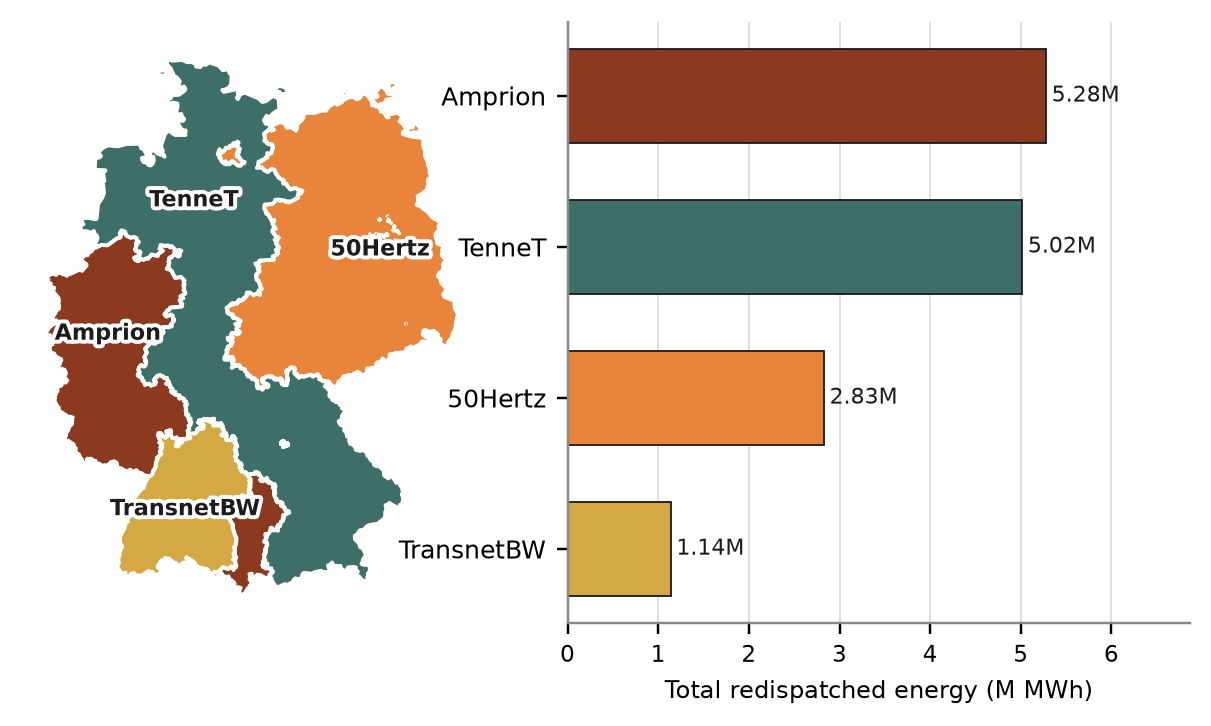
\includegraphics[width=0.85\columnwidth]{figures/Redispatch_By_Zone.png}
\caption{Real redispatch volume by German TSO control zone ($N=20{,}586$). Zone boundaries dissolved from NUTS3 district--TSO assignments \cite{ref:frysztacki2023}. Dataset context only -- not geographically resolved in the benchmark-network results.}
\label{fig:redispatch_map}
\end{figure}

\subsection{Screening and Selective Validation}
\label{sec:pipeline}
Fig.~\ref{fig:architecture} summarises the pipeline. A physics-free filter flags an event as critical if its magnitude exceeds the 95th-percentile threshold, or if its step-to-step change exceeds $1.2\sigma$ of consecutive deltas -- both are event-only features, not a two-sided band: with direction discarded in the mapping above, the event stream is a non-negative magnitude series, and a lower-tail threshold on it has no clear physical meaning, so we drop it in favour of a single high-magnitude criterion. Both thresholds are fit once from an initial 10\% calibration window of the stream (2,058 events) and then frozen for the remainder -- not recomputed from the full stream, which would let the selector condition on events that, in a real deployment, have not yet occurred. Screening is $O(1)$ per event, no power-flow solve.

Only flagged events receive a full AC solve: Newton--Raphson with $\epsilon=1\times10^{-6}$\,MVA, falling back to backward/forward sweep on non-convergence (0 solver failures observed). A deterministic hourly load-multiplier table, hashed from the run seed and event index, is applied to all feeder loads at every step.

\begin{figure}[htbp]
    \centering
    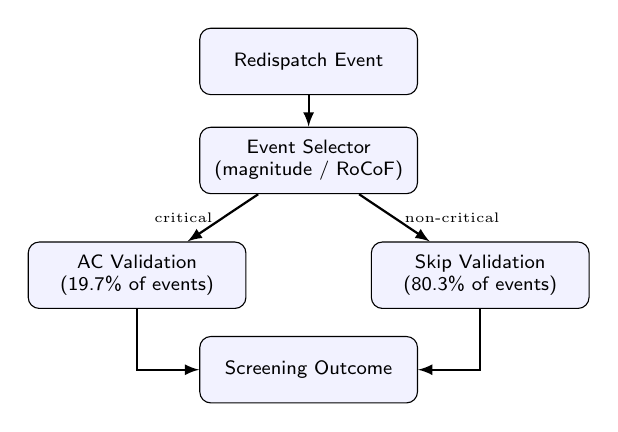
\begin{tikzpicture}[
        node distance=0.4cm,
        block/.style={rectangle, draw, fill=blue!5, text width=7.2em, text centered, rounded corners, minimum height=2.4em, font=\sffamily\scriptsize},
        line/.style={draw, -latex, thick}
    ]
        \node [block] (data) {Redispatch Event};
        \node [block, below=of data] (sel) {Event Selector\\(magnitude / RoCoF)};
        \node [block, below left=0.6cm and -0.6cm of sel] (nr) {AC Validation\\(19.7\% of events)};
        \node [block, below right=0.6cm and -0.6cm of sel] (skip) {Skip Validation\\(80.3\% of events)};
        \node [block, below=1.8cm of sel] (out) {Screening Outcome};

        \path [line] (data) -- (sel);
        \path [line] (sel) -- node[left, font=\tiny] {critical} (nr);
        \path [line] (sel) -- node[right, font=\tiny] {non-critical} (skip);
        \path [line] (nr) |- (out);
        \path [line] (skip) |- (out);
    \end{tikzpicture}
    \caption{Pipeline architecture. Thresholds are fit once from an initial calibration window and frozen; only flagged events receive AC validation. Percentages are the measured split over the real event stream ($N=20{,}586$).}
    \label{fig:architecture}
\end{figure}

\subsection{Operating-State Models}
\label{sec:opstates}
Four explicit operating-state models are evaluated, none claimed to represent the real grid: \textbf{E1}, a fixed-load control (no operating-state variation, isolates the event's own contribution); \textbf{E2}, a deterministic, hashed load table used as the main stressed evaluation regime, in which voltage violations can be systematically studied (Sec.~\ref{sec:e2stress}); \textbf{E3/E4}, independently-sourced real SimBench load profiles \cite{ref:simbench2020} (15-minute resolution, ODbL-licensed), drawn i.i.d.\ (E3) or walked in real time order (E4), at their native scale.

\subsection{A deliberately simple diagnostic regression}
\label{sec:regression}
A linear voltage-sensitivity regression, $V \approx \beta_0 + \beta_1\cdot\text{multiplier} + \beta_2\cdot P_{\mathrm{load}}$, is fit on a 70/30 split of the converged critical-path solves at each severity examined. To state the protocol explicitly: fitting happens strictly \textit{after} selector filtering, on the subset of events already flagged critical and AC-solved for the main pass -- the regression never sees a non-critical event during fitting. Training and test rows are both drawn only from this critical-path population, which never overlaps the non-critical population used for recall auditing (Sec.~\ref{sec:audit}); no row in the audited, held-out population is used for fitting at any point, and this is verified per severity, not assumed. The rule is refit fresh, independently, at each severity, because it is not a fixed algorithmic contribution being validated once -- it is a diagnostic re-estimated under each stated operating condition, exactly analogous to recalibrating a control-limit against new process data, and this refitting is what the exact split sizes in Sec.~\ref{sec:sensitivity} are reported against. The regression uses the same global load multiplier used to \textit{generate} each operating state, which is itself a controlled benchmark variable rather than an operationally available measurement (Sec.~\ref{sec:limitations}).

\subsection{Exhaustive Recall Audit}
\label{sec:audit}
Because AC validation only runs on flagged events, the selector's false-negative rate cannot be measured from the main pass alone. We separately run real AC power flow on \textit{every} event the selector calls non-critical -- not a sample -- eliminating sampling uncertainty from the false-negative rate entirely, replaying the same background load multiplier as the original pass. There is no leakage between this audit and the selector: thresholds are fixed from the calibration window alone and never adjusted using any violation outcome. The state-aware rule's catch rate (Sec.~\ref{sec:sensitivity}), unlike the exhaustively-audited false-negative rate, is a property of the regression's behaviour on held-out violations, so we report it with a Wilson-score 95\% CI \cite{ref:wilson1927}, which avoids the normal approximation's boundary failures at the small violation counts observed near onset.

\subsection{Latency Measurement}
\label{sec:latency_method}
Reported cycle times distinguish \textit{screening latency} (the $O(1)$ filter, sub-millisecond regardless of criticality), \textit{AC validation latency} (Newton--Raphson on flagged events only), and \textit{end-to-end operational latency} (which we do not measure -- our timing covers software execution on one machine, not a full control-loop deadline including telemetry and actuation). The AC solver's JIT-compiled kernels (internal to \textit{pandapower}, via \textit{numba}) are explicitly warmed with one throwaway solve before timing begins, so the one-time compilation cost is reported separately (Sec.~\ref{sec:results}) rather than misattributed to whichever event happens to run first. Five independent process invocations are used throughout, each measured cold.

\subsection{Reproducibility}
All results use a fixed seed (42); package versions, platform, and a SHA-256 hash of the input CSV are captured in a machine-readable header at run time (Python 3.13.14, pandapower 3.5.4, \textit{numba} 0.66.0; Apple M5, 10 cores, macOS/Darwin 25.6.0 -- shared, general-purpose hardware, not an isolated benchmarking environment). Violation and recall counts are deterministic given the seed and pinned software; wall-clock cycle times are not seed-controlled and vary with machine load. Source code and the exact input dataset will be published upon acceptance.\footnote{Repository: \url{https://github.com/omari91/rt-grid-streaming-engine}}

% --- RESULTS ---
\section{Results}
\label{sec:results}

\subsection{Event-Only Screening: Recall and Precision (RQ1)}
\label{sec:screening_result}
Under the E2 evaluation regime, the selector flags 4,055 of 20,586 events (19.7\%) as critical; AC validation converges on all 4,055 (0 solver failures) and confirms 239 voltage-limit violations. An exhaustive audit of the remaining 16,531 non-critical events -- not a sample -- finds a further 1,305 violations (7.9\% false-negative rate). The total violation population across the full stream is exactly 1,544, giving an exact overall recall of $\mathbf{15.5\%}$.

Recall alone understates the trade-off: of the 4,055 AC validations the selector triggers, only 239 find a violation -- precision of $\mathbf{5.9\%}$, meaning 94.1\% of triggered AC validations are non-violations (false-discovery rate; see Table~\ref{tab:recall}).
%a false-positive rate of $20.0\%$, and a false-discovery rate of $94.1\%$ (Table~\ref{tab:recall}). 
Roughly 19 in 20 selective validations this screen triggers come back clean.

\begin{table}[htbp]
\caption{Event-only screening: exhaustive audit results (E2)}
\label{tab:recall}
\centering
\begin{tabular}{@{}lc@{}}
\toprule
\textbf{Metric} & \textbf{Value} \\ \midrule
Confirmed violations (critical path, exact) & 239 \\
Confirmed violations (non-critical, exact) & 1{,}305 \\
Total violations, full population (exact) & 1{,}544 \\
Recall (exact) & 15.5\% \\
Precision (of AC validations triggered) & 5.9\% \\
False-positive rate & 20.0\% \\
False-discovery rate & 94.1\% \\ \bottomrule
\end{tabular}
\end{table}

This precision-recall trade-off is not an artefact of where the magnitude threshold happens to be set. Sweeping the selector's percentile threshold from the 90th to the 99th (exhaustive audit repeated at each point, everything else unchanged) shows precision essentially flat at $5.8$--$6.0\%$ throughout, while recall falls monotonically as the threshold tightens, from $17.4\%$ (90th) to $14.3\%$ (99th; Table~\ref{tab:threshold_sens}). Moving the threshold trades a little recall for no meaningful precision gain -- consistent with Sec.~\ref{sec:why_fails}'s finding that magnitude itself, not this particular cutoff on it, is the weak signal.

\begin{table}[htbp]
\caption{Threshold sensitivity: selector percentile vs.\ precision/recall (E2, exhaustive audit at each point)}
\label{tab:threshold_sens}
\centering
\small
\begin{tabular}{@{}lccc@{}}
\toprule
\textbf{Percentile} & \textbf{$n_{\mathrm{critical}}$} & \textbf{Precision} & \textbf{Recall} \\ \midrule
90th & 4,653 & 5.8\% & 17.4\% \\
93rd & 4,302 & 5.8\% & 16.2\% \\
95th (default) & 4,055 & 5.9\% & 15.5\% \\
97th & 3,843 & 6.0\% & 15.1\% \\
99th & 3,603 & 6.0\% & 14.3\% \\ \bottomrule
\end{tabular}
\end{table}

\subsection{Why Event-Only Screening Fails (RQ2)}
\label{sec:why_fails}
A control condition isolates the event's own contribution: the same stream and selector, but feeder loads held at nominal CIGRE values (no operating-state variation). Across all 4,055 flagged events, AC validation finds \textbf{zero} violations; minimum voltage is 0.926\,p.u. (mean 0.930), well clear of 0.90\,p.u. regardless of event magnitude. No redispatch event in this real dataset, however extreme, is sufficient on its own to cause a violation -- every confirmed violation requires operating-state variation.

A regression against the 4,055 converged critical-path solves confirms why: $V \approx 1.038 - 0.110\cdot\text{multiplier} + 0.010\cdot P_{\mathrm{load}}$, fit on a 70/30 split with training $R^2=0.992$ and held-out $R^2=0.992$ -- the two are indistinguishable, %so this is not overfit. 
showing no evident train/test degradation.
Background loading correlates with voltage at $r=-0.99$; the event's own magnitude correlates at only $r=0.06$ -- consistent with classical distribution voltage-sensitivity theory \cite{ref:baran_wu1989}: aggregate feeder loading acts on every downstream bus simultaneously, while one generator's injection is comparatively local. The selector conditions on magnitude and rate-of-change -- precisely the weaker signal, which is why most confirmed violations occur among events it does not flag rather than among the ones it does.

\subsection{Does This Survive Independent Load Data? E2 as a Stress Regime (RQ2)}
\label{sec:e2stress}
E2's loading-voltage correlation replicates closely under both independent SimBench conditions ($r=-0.99$, E3 and E4 individually) -- not an artifact of E2's own hashed construction. The violation \textit{count} does not replicate: E3/E4 both find \textbf{zero} violations among the same 4,055 critical events that yield 239 under E2, at native scale. We traced this to source rather than leaving it unexplained: E2's table derives from seasonal CIGRE-network load curves simulated by Porsinger et al.\ \cite{ref:porsinger2017} and subsequently curated into specific multi-day test windows by a public repository; the window used here is documented by its curator as producing network overloads and voltage-limit problems, peaking $26\%$ above this network's own documented peak-load specification \cite{ref:rudion2006} -- a genuine overload condition by construction, not an incidental one. E2 is therefore best understood as \textbf{a controlled, stressed evaluation regime} in which violations can be systematically studied, not a claim about typical operating severity. %real, representative load data never exceeds the documented peak
The native-scale SimBench profiles used here do not exceed the benchmark's documented peak, which is why E3/E4 do not violate at native scale. The mechanism linking operating state to voltage is reproduced under independent data; the prevalence of violations is highly sensitive to how severely loading is stressed.

\subsection{State-Aware Screening Across Stress Levels (RQ2)}
\label{sec:sensitivity}
The finding above motivates testing state-aware screening across a range of severities, not one. Here, state-aware means conditioned on the benchmark's known global loading multiplier; this is a controlled proxy for an operational state estimate, not a directly deployable measurement.

The rule from Sec.~\ref{sec:regression}, refit fresh %and applied strictly out-of-sample at each severity, was evaluated exhaustively 
at each severity and evaluated on the disjoint non-critical population, was applied exhaustively
(full 16,531-event non-critical census, not a sample) at E2's own severity plus two further points obtained by scaling real SimBench shape uniformly -- a transparent, pre-declared multiplier ($1.00$--$2.00\times$) calibrated against this network's documented peak, not chosen to produce a particular result: %: violations first appear at $1.35\times$; we audit $1.50\times$ and $1.75\times$, past this onset. 
E2 corresponds to a separate curated stress regime at $1.26\times$ the documented peak. In the independent SimBench-shape sweep, violations first appear at $1.35\times$; we therefore audit $1.50\times$ and $1.75\times$, both beyond this onset.
%At every severity, the 70/30 split of the 4,055-event critical-path population produces the same $n_{\mathrm{train}}=2{,}838$, $n_{\mathrm{test}}=1{,}217$ -- confirming the fit always draws from the full critical-path population at that severity, never from the non-critical population being audited.

Because the event-only selector is independent of operating-state severity, the same 4,055 event IDs form the critical-path population at every severity. 
At every severity, these are split 70/30, yielding $n_{\mathrm{train}}=2{,}838$ and $n_{\mathrm{test}}=1{,}217$; neither the training nor held-out set overlaps the non-critical population used for the recall audit.

%State-aware screening provides limited detection improvement near violation onset but becomes substantially more effective under severe stress: catch rate is statistically flat between $1.26\times$ and $1.50\times$ (20.5\% vs.\ 26.0\%, heavily overlapping 95\% CIs) and jumps sharply by $1.75\times$ (74.3\%, CI $[70.8,77.5]\%$, not overlapping either earlier point; Table~\ref{tab:sensitivity}). 
State-aware screening provides limited detection improvement in the E2 stress regime and near the onset region, but becomes substantially more effective under severe stress: violation recall is 20.5\% at E2 ($1.26\times$), 26.0\% at $1.50\times$, and jumps to 74.3\% at $1.75\times$, compared with 20.5\% and 26.0\% at the lower tested severities (Table~\ref{tab:sensitivity}).

An earlier in-sample evaluation suggesting near-complete recall was discarded after leakage was identified; %all results reported here use the corrected, out-of-sample protocol.
the results reported here use the corrected held-out fitting and population-separated evaluation protocol.

\begin{table}[htbp]
%\caption{State-aware screening recall by severity, as a multiple of documented peak load (full non-critical population audited exhaustively at each point)}
\caption{Violation recall by severity, as a multiple of documented peak load. Recall denotes the fraction of confirmed voltage violations in the audited non-critical population that are correctly flagged by the state-aware screen; the full non-critical population is audited exhaustively at each point.}
\label{tab:sensitivity}
\centering
\footnotesize
\setlength{\tabcolsep}{3pt}
\begin{tabular}{@{}lcccc@{}}
\toprule
\textbf{Severity} & \textbf{FN rate} & \textbf{Precision} & \textbf{Violation Recall \%} & \textbf{95\% CI (\%)} \\ \midrule
$1.26\times$ (E2) & 7.9\% & 5.9\% & 20.5\% & 18.4--22.7 \\
$1.50\times$ (scaled) & 0.4\% & 0.3\% & 26.0\% & 17.3--37.1 \\
$1.75\times$ (scaled) & 3.9\% & 3.2\% & \textbf{74.3\%} & \textbf{70.8--77.5} \\ \bottomrule
\end{tabular}
\end{table}

\subsection{Computational Cost (RQ3)}
\label{sec:cost}
Screening is sub-millisecond regardless of criticality (median 0.003\,ms). With redundant Newton--Raphson solves deduplicated (one solve per unique dispatch value, not per downstream consumer of the result) and the AC solver's JIT compilation explicitly warmed before timing begins, critical-path AC validation has a median cycle time of 4.7\,ms (p95 4.9\,ms, p99 5.1\,ms). The one-time JIT compilation cost, isolated from this measurement, is 795--815\,ms across five independent runs -- a startup cost, not a steady-state one.

%Across five independent standalone runs, selective validation misses the 20\,ms software-execution deadline on exactly \textbf{1 of 4,055} critical events (0.025\%) in every run 
Each of five independent runs has exactly one event exceeding the 20\,ms threshold ($1/4055 = 0.025\%$ per run, see Fig.~\ref{fig:cycle_trace}). The missing event is not fully deterministic -- event 9251 in four of five runs, a different event in the fifth -- consistent with observed machine jitter on shared, general-purpose hardware, not a real-time guarantee: we report sub-20\,ms AC validation/software execution latency on the tested platform under the tested conditions, not real-time verification, and we did not measure end-to-end operational latency including telemetry and actuation (Sec.~\ref{sec:latency_method}).

\begin{table}[htbp]
\caption{Cycle-time distribution by path, JIT warm-up excluded (representative run)}
\label{tab:latency}
\centering
\begin{tabular}{@{}lccc@{}}
\toprule
\textbf{Path} & \textbf{Median (ms)} & \textbf{p95 (ms)} & \textbf{Misses} \\ \midrule
Non-critical ($n=16{,}531$) & 0.003 & 0.005 & 0/16{,}531 \\
Critical ($n=4{,}055$) & 4.7 & 4.9 & 1/4{,}055 \\ \bottomrule
\end{tabular}
\end{table}

\begin{figure}[htbp]
    \centering
    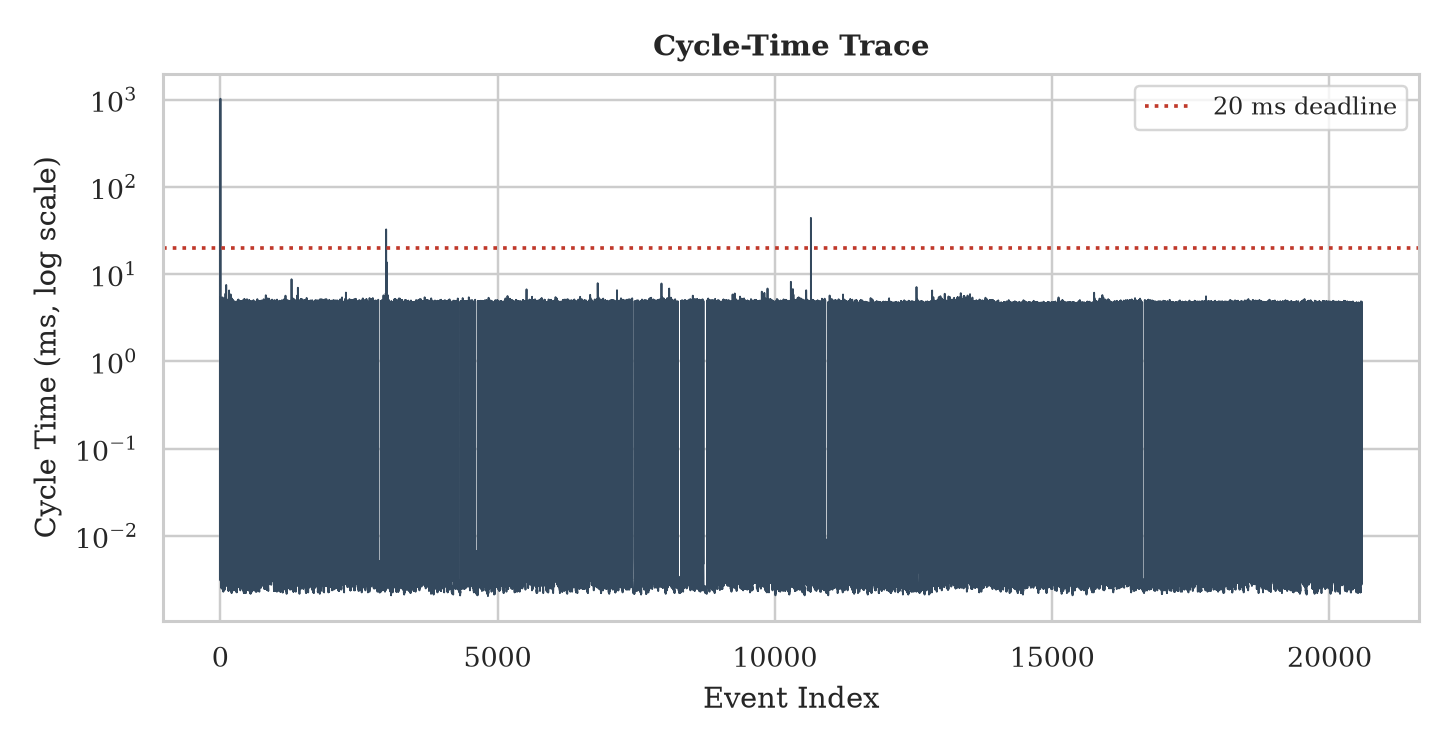
\includegraphics[width=0.9\columnwidth]{figures/Cycle_Time_Trace.png}
    \caption{Per-event cycle time ($N=20{,}586$, log scale, JIT warm-up excluded) against the 20\,ms software-latency threshold. The critical-path band sits almost entirely below it.}
    \label{fig:cycle_trace}
\end{figure}

The curtailment mechanism tested for closed-loop control did not activate within the target generator's operating range on this dataset, so we do not report it as a substantive controller comparison (Sec.~\ref{sec:limitations}).

% --- CONCLUSION ---
\section{Limitations and Conclusion}
\label{sec:conclusion}

\subsection{Limitations}
\label{sec:limitations}
Redispatch events are mapped to a single generator's setpoint, not the real, distributed set of assets a TSO instruction would affect; this is a major external-validity limitation we do not attempt to resolve with a new experiment under this deadline, and the $r=0.06$ event-magnitude correlation should not be generalized to real-world redispatch broadly. Clipping to 1.5\,MW affects 0.02\% of events -- negligible. The global loading multiplier used to define operating-state severity is a controlled state variable in this benchmark, not an operationally observable measurement; a real implementation would require this signal from state estimation or feeder telemetry. E2 is a documented, curated overload regime, $26\%$ above this network's own specified peak, useful for systematically studying violations but not representative of typical severity; specific violation counts and catch rates are sensitive to the operating-state model assumed, even though the underlying loading-dominates-magnitude mechanism is not. Voltage states come from AC simulation on a benchmark network, not measured feeder telemetry. The 20\,ms figure is an experimental software-latency threshold, not a guaranteed real-time deadline, and latency was measured on one shared machine, not dedicated real-time hardware. The tested closed-loop curtailment mechanism did not activate within the generator's operating range and was not meaningfully evaluated as a control comparison. Broader network-scale validation beyond this one 15-bus benchmark remains future work. Modern DMS/SCADA platforms already embed an AC solver for other functions (state estimation, contingency analysis), so the screening layer evaluated here is additive software -- a magnitude/rate-of-change filter ahead of an existing solver call -- rather than new infrastructure; deployment does not require new sensing, since it consumes the same instruction stream and background-loading signal such platforms already carry. The open question for an operator evaluating adoption is calibration, not solver availability: the state-aware threshold would need re-fitting on a utility's own network and load data, closer in scope to an existing periodic load-flow planning study than to a new monitoring deployment, before being trusted operationally rather than transferred as-is from this benchmark.

\subsection{Conclusion}
Event information alone is an insufficient screening proxy: it achieves 15.5\% recall at 5.9\% precision against an exhaustive AC-validated ground truth. Operating state substantially changes screening performance under the tested benchmark conditions: a fixed-load control finds zero violations from event information alone, and state-aware screening's value is concentrated well past the onset of violations (74.3\% at $1.75\times$) rather than near it (20.5\% at $1.26\times$). Selective AC validation is computationally inexpensive on the tested platform (0.025\% software-latency threshold exceedance rate, JIT cost isolated), but broader physical and real-time validation is still required before any operational claim beyond this benchmark.

\subsection{Conclusion}
Event magnitude alone is an insufficient screening proxy: it achieves 15.5\% recall at 5.9\% precision against an exhaustive AC-validated ground truth. Operating state substantially changes screening performance: a fixed-load control finds zero violations from event magnitude alone, and state-aware screening's value is concentrated well past the onset of violations (74.3\% at $1.75\times$) rather than near it (20.5\% at $1.26\times$). Selective AC validation is computationally inexpensive on the tested platform (0.025\% deadline-miss rate, JIT cost isolated), but broader physical and real-time validation is still required before any operational claim beyond this benchmark.

{\footnotesize
\bibliographystyle{IEEEtran}
\bibliography{reference}
}
\end{document}
